
\documentclass[nototal]{beamer}
\mode<presentation>
{
  \usetheme{Madrid}
  \setbeamercovered{transparent}
}

\usepackage{verbatim}
\usepackage{fancyvrb}
\usepackage[english]{babel}
\usepackage[latin1]{inputenc}
\usepackage{times}
\usepackage{tikz}
\usepackage[T1]{fontenc}
\usepackage{graphicx} %sjr added
\graphicspath{{figures/}}
\usepackage{hyperref}

\author[S. Rey]{\textsc{Sergio Rey}}
\institute[ASU]{\textbf{GPH 483/598}\\\textbf{Geographic Information Analysis}\\School of Geographical Sciences and Urban Planning\\Arizona State University\\Fall 2010}
\title[Spatial Data]{Spatial Data}
\subtitle{}
\date[GPH 483/598]{}

% Delete this, if you do not want the table of contents to pop up at
% the beginning of each subsection:
\AtBeginSubsection[]
{
  \begin{frame}<beamer>
    \frametitle{Outline}
    \tableofcontents[currentsection,currentsubsection]
  \end{frame}
}


% If you wish to uncover everything in a step-wise fashion, uncomment
% the following command: 
%\beamerdefaultoverlayspecification{<+->}
\begin{document}
\begin{frame}
  \titlepage
\end{frame}


\begin{frame}{Outline}
  \tableofcontents[pausesections]
\end{frame}

\section{Introduction}
\begin{frame}
  \begin{columns}[t]
    \column{.5\textwidth}
    \frametitle{First one}
    \begin{block}{Block title}
      \begin{itemize}
	\item There one
	\item to
	\item three
	\item four
	\item five
      \end{itemize}
    \end{block}

    \column{.5\textwidth}
    \begin{block}{Second block}
      \begin{itemize}
	\item first
	\item second
	\item third
	\item fourth
      \end{itemize}
    \end{block}
  \end{columns}
\end{frame}

\subsection{Spatial Data}


\frame{
\frametitle{Split screen}
\begin{columns}
  \begin{column}{3cm}
    \begin{itemize}
      \item<1-> a
      \item<3-> b
      \item<5-> c
    \end{itemize}
    \vspace{3cm} 
  \end{column}
  \begin{column}{7cm}
    \begin{overprint}
      \includegraphics<2>[width=7cm]{single1.png}
      \includegraphics<4>[width=7cm]{single2.png}
      \includegraphics<6>[width=7cm]{single3.png}
    \end{overprint}
  \end{column}
\end{columns}}

\subsection{Nonspatial Data}

\begin{frame}
  \frametitle{Figure}
  \begin{center}
    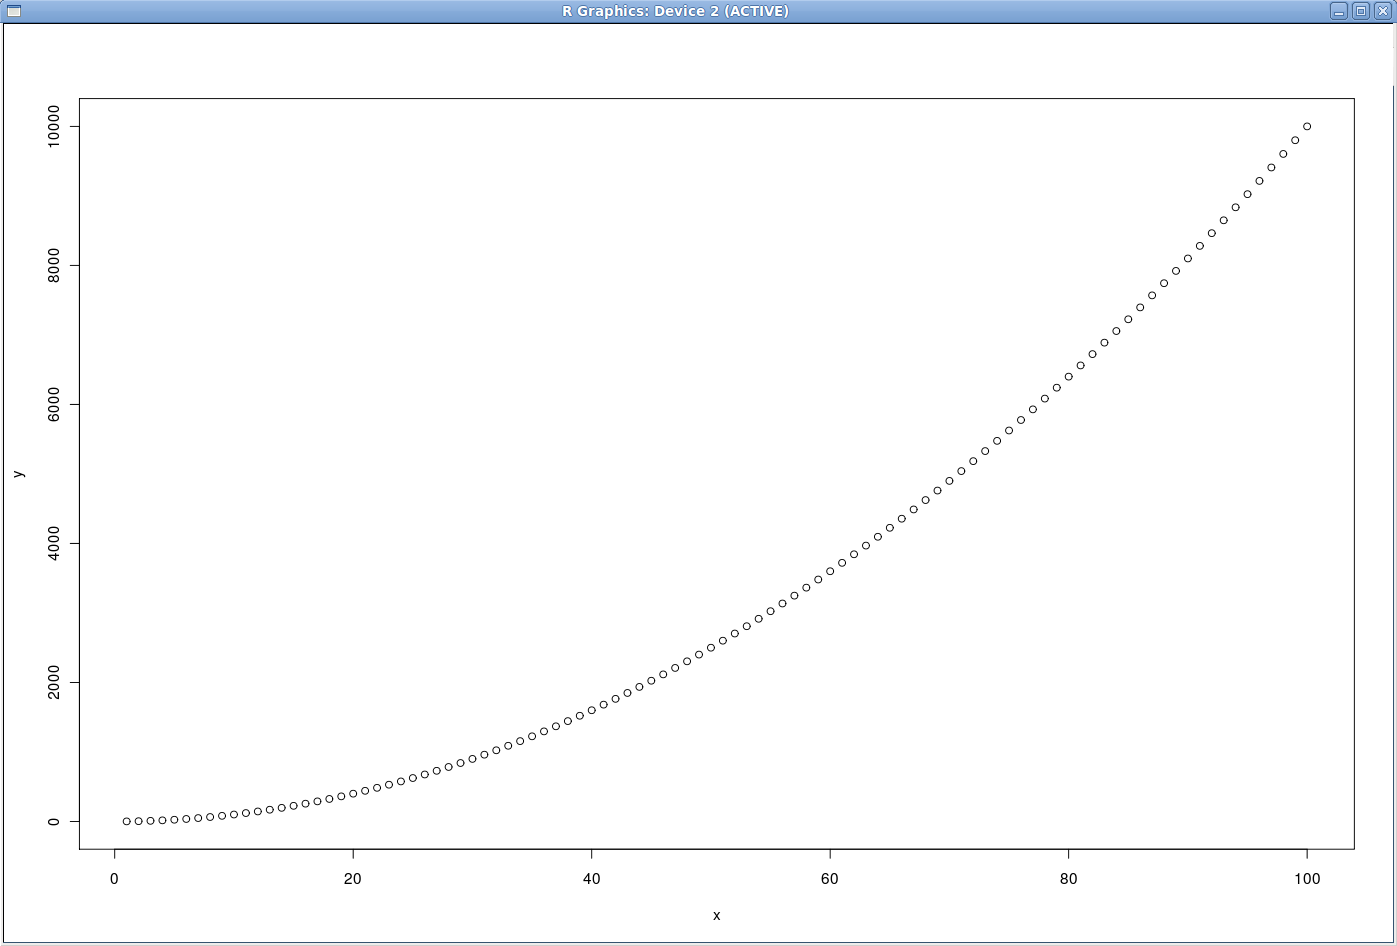
\includegraphics[width=.85\linewidth]{screenshot_003.png}
  \end{center}
\end{frame}

\begin{frame}
  \frametitle{Figure}
  \begin{center}
    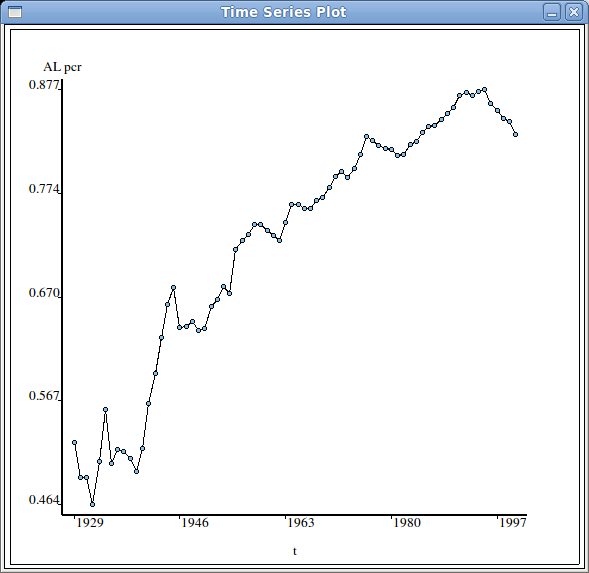
\includegraphics[width=.85\linewidth]{starsnew.png}
  \end{center}
\end{frame}


\section{Representation}
\subsection{Change of support}
\subsection{MAUP}

\end{document}

